\section{Introducción}

\subsection{1.1 Motivación y Problemática}

Aunque los métodos de fabricación convencionales han servido de columna vertebral para la industria satelital durante décadas, su rigidez inherente limita drásticamente las posibilidades de optimización en un entorno donde cada gramo cuenta. Resulta particularmente llamativo observar cómo la escalada de constelaciones de bajo órbita para telecomunicaciones ha intensificado la presión por reducir masa, costos de lanzamiento y tiempos de ensamblaje, sin comprometer la integridad estructural ni el rendimiento RF.

Uno de los desafíos persistentes radica en la multiplicidad de piezas y uniones que caracterizan los diseños tradicionales. Estas configuraciones no solo elevan el riesgo de fallos en vibración y fatiga, sino que complican el mantenimiento y aumentan los plazos de integración. En este contexto, la fabricación aditiva emerge como una alternativa capaz de consolidar componentes y generar geometrías imposibles por vías sustractivas. 

Boschetto et al. demostraron de forma convincente esta potencialidad al rediseñar estructuras de plataforma satelital mediante estructuras lattice internas fabricadas por Powder Bed Fusion con láser (PBF-LB/M), logrando reducciones de masa entre 4\% y 28\% mientras se mantenían las frecuencias dinámicas requeridas \cite{Boschetto2023}. Tales resultados no representan meras mejoras incrementales, sino un cambio paradigmático en la forma de concebir hardware espacial. 

Dalmarco et al., por su parte, destacan que la reducción de masa y costos constituye uno de los principales drivers de adopción de AM en el sector espacial europeo, aunque matizan que los procesos de calificación siguen representando una barrera significativa \cite{Dalmarco2026}.

\begin{table}[h]
\centering
\caption{Comparación entre fabricación tradicional y aditiva en componentes satelitales}
\label{tab:comparacion_trad_vs_am}
\begin{tabular}{lcc}
\hline
\textbf{Aspecto} & \textbf{Tradicional} & \textbf{Fabricación Aditiva} \\
\hline
Número de piezas & Alto & Bajo (consolidación) \\
Masa & Referencia & -15\% a -40\% \\
Tiempo de ensamblaje & Elevado & Reducido \\
Complejidad geométrica & Limitada & Alta \\
Costo de lanzamiento & Alto & Potencialmente menor \\
\hline
\end{tabular}
\end{table}

\begin{figure}[h]
\centering
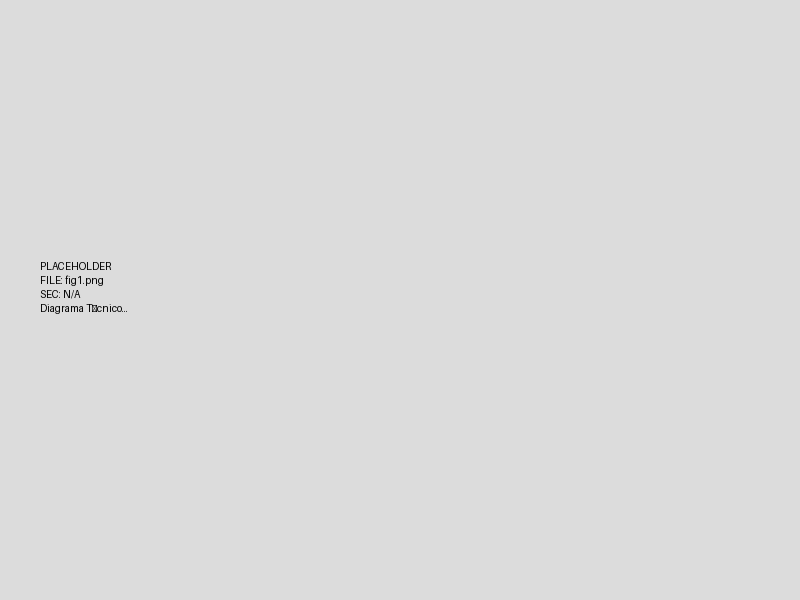
\includegraphics[width=0.85\linewidth]{fig1.png}
\caption{Evolución de la masa específica en plataformas satelitales de telecomunicaciones (kg/kW). Se observa la tendencia a la baja impulsada por tecnologías de fabricación aditiva desde 2018.}
\label{fig:evolucion_masa}
\end{figure}

\subsection{1.2 Objetivos e Hipótesis}

Particularmente revelador es el potencial que ofrece la fabricación aditiva cuando se aplica no solo a estructuras portantes, sino también a componentes RF críticos en bandas Ku y Ka. Talpur et al. ofrecen en su revisión exhaustiva una visión actualizada de cómo las técnicas AM permiten una flexibilidad de diseño sin precedentes en antenas y alimentadores para SATCOM, reduciendo costos y mejorando prestaciones en entornos donde la integración multifuncional resulta clave \cite{Talpur2025}.

La hipótesis central de este trabajo sostiene que una aproximación sistemática de Design for Additive Manufacturing (DfAM) aplicada a plataformas minisatélite de telecomunicaciones puede lograr reducciones simultáneas de masa superiores al 25\%, tiempos de ensamblaje inferiores en un 40\% y mejoras en mantenibilidad, sin penalizar el comportamiento estructural ni electromagnético. Esta hipótesis se sustenta tanto en evidencia experimental previa como en las capacidades actuales de simulación multidisciplinaria.

\subsection{1.3 Alcance y Estructura del Artículo}

Lejos de pretender una cobertura universal, el presente artículo se centra en aplicaciones para satélites de telecomunicaciones en órbita baja, con énfasis en estructuras primarias, brackets funcionales y componentes RF. Aunque reconoce las limitaciones actuales en calificación espacial y disponibilidad de materiales certificados, explora caminos realistas para superarlas.

El resto del documento se organiza de la siguiente manera. La Sección 2 revisa el estado del arte. La Sección 3 detalla la metodología DfAM propuesta. Posteriormente, la Sección 4 presenta los resultados obtenidos, mientras que la Sección 5 discute sus implicaciones. Finalmente, las conclusiones y líneas de trabajo futuro cierran el artículo.